\documentclass[../main2.tex]{subfiles}
%if compiling standalone, rootdir wil be previous folder,
%if compiling main document, rootdir will already be set by main file
\providecommand{\rootdir}{..}

\begin{document}

\subsection{Dynamic Range}
\begin{itemize}
\item Peak
\item RMS
\item Crest factor
\item VU
\item EBU 3341 
\item EBU Tech 3342
\item ITU recommendation BS 1770
\item http://productionadvice.co.uk/how-to-avoid-over-compressing-your-mix/
\item http://www.soundonsound.com/sos/sep11/articles/loudness.htm
\begin{itemize}
\item there is no official definition for it, and it may be confused with the dynamic range of a recording medium, which is basically the difference between the highest and lowest level it can handle.
\end{itemize}
\end{itemize}

http://www.analog.com/en/education/landing-pages/001/relationship-data-word-size-dynamic-range.html#Appendix_-_References


\subsection{Envelope}
How does the envelope map to the dynamic range?

Envelope vs finestructure

Philosophy of envelope detection => feed forward side chain

Inherent nonlinear operation that is not well defined, since no mathematical operaton is known to the authors that separates envelope from fine structure the same way the human ear hears it (Source Cochlia site claiming this is possible to do...)

Freq of modulated signal
Freq of ideally compressed signal

Freq of modulated chord

Constructing a signal with as low ambiguity as possible

Sine and square?

Stone and Moore => Guianuulis
Slight shift in FES meaning => FIES

\subsection{Envelope Detection}
To change the dynamic range, it seems reasonable to know what it is to begin with. This is the purpose of envelope detection, envelope following or envelope creation.

Envelope construction (source TAES?) better term.
Detector approaches

\subsection{Metrics}
FES vs THD

dividing out the input finestructure. Show freq. Show example envelope with distortion. => the envelope takes all distortion in the FES, even though it may not be heard as the wrong envelope but as distorted finestructure.

How to measure THD? Begin and end phenomenon will look like distortion, but sound like envelope modulation.


Stone and Moore, uses FES and ECR to characterise compression incl. parameter settings, and test correllation to speach intelligability.

Giannoulis use the metrics to compare different compressors, with same settings. Buuu!

Show limits to the metrics, eg. no compression => perfect FES etc.
AND that no compressor no matter how good it is, can achieve ideal FES, since it BY DEFINITION changes the envelope shape.

Define an ideal compressor that actually compresses the dynamic range (defined from envelope) but still has perfect FES (Above threshold!), THD and ECR.
On certain signals: with well defined envelope. 

Measure euclidian norm to this ideal compressor




Det finns massa faktorier, artefakter, fel, etc som kan "låta bra". Detta motsäger dock inte behovet av en transparent grund att bygga vidare på. (se Frindle)

Givet att vi har lyckats definiera transparens i sammanhanget => Borde detta ge en bra första indikation på en kompressors prestanda.
Det kan mäta bra men inte vara speciellt transparent andra sammanhang. (med mer komplicerad fine str) Men det verkar osannolikt att den skulle mäta dåligt och vara transparent på mer komplicerade signaler? Lyssnar tester behövs för att kvantifiera detta påstående. Psychoacoustics.


\subsection{Compressor parameters}
Different designs have different sets of parameter settings, which make comparisons difficult. The following distiction is made. 

Defining which we regard as 
\begin{itemize}
\item \textbf{defining compression} - gain computer: Treshold, Ratio, Make-up gain
\item \textbf{artistic parameters} - gain smoothing: attack, release, hold etc
\item \textbf{unfortunate parameters, necessary evils} - Envelope detection params: attack, release, hold, TAV, window width etc. the user should not ideally control those (at least not when the goal is transparent compression, the artistic goals can of course make these useful) These are often not visible to the user, but may be predefined to give the compressor it's characteristic sound.
\end{itemize}

In theory, such a clean separation is possible, but in practice all params have a complicated interplay. Knee smoothing for example may be used to change the definition of compression region, or to mitigate artifacts in the envelope detection/gain smoothing.
Another example is the Gain smoothing, which may be used to change the behaviour from ideal to artistic, or simply as a second filter mitigating artifacts in the envelope detection.

When comparing different compressors we do the following:
\begin{itemize}
\item The parameters defining compression are static. 
\item The necessary evil parameters, are optimised numerically for each input signal, to make the comparisons as fair as possible.
\item The artistic parameters are omitted AND or optimised numerically, this is to see if they can be used to mitigate artifacts and in that case make comparisons fairer, but not hide the fact that the user might be forced to make a judgement call between for example artifact considerations such as motorboating, and artistic wants such as fast recovery in the case of release time (source Stickvoort).
\end{itemize}

\subsection{Peak detectors}
\begin{itemize}
\item Peak detectors
\item RMS detectors
\item Where to put window detectors?
\end{itemize}
Difference between Peak and RMS
Peak with linear filter: Asin => 2A/pi, Asquare => A
RMS with linear filter Asin =>  A/sqrt(2), Asquare => A
Peak with nonlinear filter: Asin => ocillates under A, Asquare=> A
RMS with nonlinear filter: Asin => oscillates under A, Asquare=> A

So it's not the squaring operation that makes the difference between peak and RMS!
It is the nonlinear vs the linear filter!

Thus we can implement 3 different types of compressors
\begin{itemize}
\item defining the envelope as RMS value: - only RMS with LINEAR filter ok as envelope detector
\item defining the envelope as peak value: Peak with NONlinear filter, or RMS with NONlinear filter
\item defining the envelope as abs-mean-value: - only peak with LINEAR filter ok. But what does this mean? Discard as there is no clear meaning to this level.
\end{itemize}
As it turns out, RMS with NONlinear filter is a BETTER peak detector than ABS with NONlinear filter, since the filtering is done on fewer harmonics, instead of filtering a lot of harmonics and then squaring. :) :) :) :)

http://www.uaudio.com/webzine/2005/july/text/content2.html

We will use the convention to calculate signal level in dB relative to Full Scale, that is $20 \log_{10} A/A_0$ where $A_0$ is the largest possible amplitude, which we will define as $A_0 = 1$ as common in floating point environments.
When measuring average rms levels, although not the standard recommended by  AES Standard AES17-1998, we will use the rms of a square wave as reference when measuring dB FS. So a sine wave with a peak value of 0 dB FS, will have an rms of -3 dB FS. This is for clarity, as the rms value of sine wave actually is $1/\sqrt(2)$ and thus $-3$ dB below the highest possible average rms of 1 (achieved by a square wave). 


\begin{figure}
\centerline{
	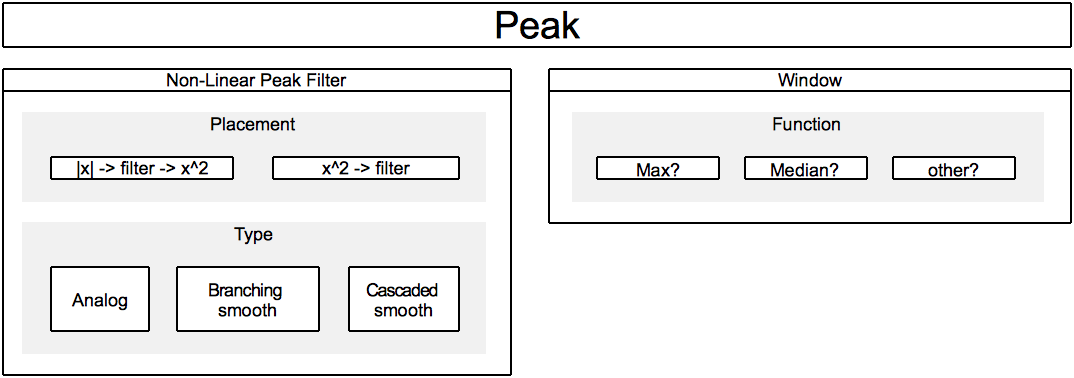
\includegraphics[width=\textwidth]{\rootdir/pictures/peak_detector_designs.png}
}
\caption{Peak detector design choices}
\label{fig:peak_detector_design}
\end{figure}

\begin{figure}
\centerline{
	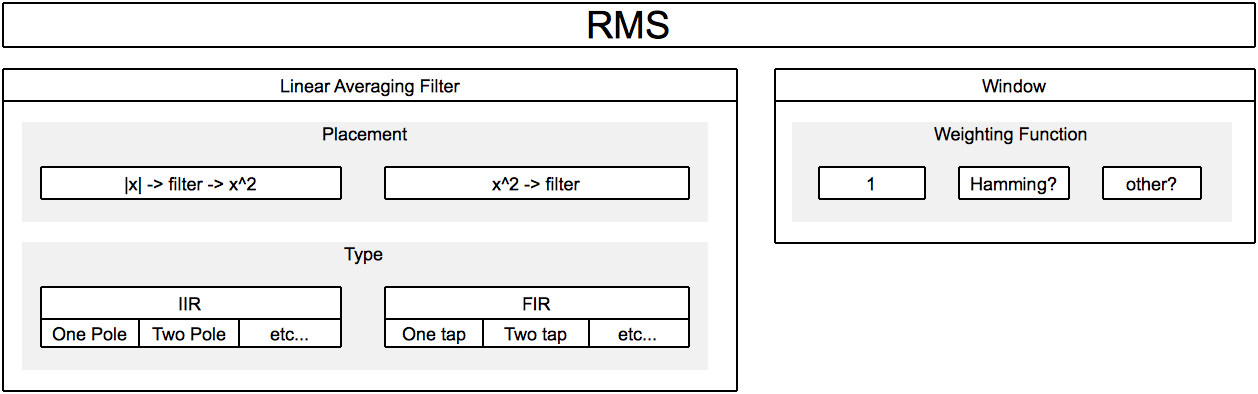
\includegraphics[width=\textwidth]{\rootdir/pictures/rms_detector_designs.png}
}
\caption{RMS detector design choices}
\label{fig:rms_detector_design}
\end{figure}

Questions:
\begin{itemize}
\item What does a compressor do?
	\begin{itemize}
	\item Dynamic Range, not signal to noise ratio, but rather Level variability
	\item Sound Level (dBFS, peak and rms), and Loudness
	\item Envelope
	\end{itemize}
	
\item What design choices are recommended in scientific literature?
	\begin{itemize}
	\item Feed forward vs Feedback
	\item Peak vs RMS
	\item Gain computer
	\item Gain smoothing
	\end{itemize}
	
\item What is the design goal? Does an ideal compressor exist?
	\begin{itemize}
	\item Transparent compression
	\item Concept of Envelope and Finestructure
	\item Not well defined
	\item The story of FES and ECR, Stone and Moore vs Giannoulis
	\item THD?
	\item Definition of Ideal compression from above metrics adjusted
	\item most "artifacts" from wrong parameter settings, optimize!
	\end{itemize}
	
\item Are some designs better than others according to this criteria?
	\begin{itemize}
	\item Envelope detection, Peak and RMS
	\item The effect of upsampling
	\item Gain smoothing as user param and interacting with envelope detection
	\item Results for the whole compressor
	\end{itemize}

\end{itemize}

\section{Method}

\begin{itemize}
	\item the story of Stone and Moore vs Giannoulis
	\item Slight shift in FES meaning => FIES
	\item THD?
	\item Inherent nonlinear operation that is not well defined, since no mathematical operaton is known to the authors that separates envelope from fine structure the same way the human ear hears it (Source Cochlia site claiming this is possible to do...)
	\item Freq of modulated signal
	\item Freq of ideally compressed signal
	\item Freq of modulated chord

	\item Definition of Ideal compression from metrics previously discussed
	\item Constructing a signal with as low ambiguity in envelope vs fine strucutre as possible
	\item only Sine as fine strucutre? True square wave? Other?

	\item The inherent nonlinearity of the compressor motivates both measuring the parts them selves, AND their interaction.
	
	\item Level detectors, peak and RMS
	\item The effect of upsampling
	
	\item Only take the absolute value and test 

	\item most "artifacts" from wrong parameter settings, optimize!
\end{itemize}


\end{document}